\documentclass[notitlepage,cs4size,punct,oneside]{ctexrep}

% default paper settings, change it according to your word
\usepackage[a4paper,hmargin={2.54cm,2.54cm},vmargin={3.17cm,3.17cm}]{geometry}

\usepackage{amsmath,amssymb,amsthm}
\usepackage{titlesec}

% 公式编号的计数格式, 在章内计数
\numberwithin{equation}{chapter}

% set the abstract format, need abstract package

\usepackage[runin]{abstract}
\usepackage{algorithm}
\usepackage{algpseudocode}
\usepackage{booktabs}
\usepackage{graphicx}
\usepackage{float} % 图片和表格定位
\usepackage{subfigure} % 子图包
\usepackage{xcolor}





\usepackage[pdfborder={0 0 0},colorlinks=true,linkcolor=blue,CJKbookmarks=true, unicode=true]{hyperref}
%若要用LATEX编译, 请用下面的命令替代上述命令:
% \usepackage[dvipdfm,pdfborder={0 0 0},colorlinks=true,linkcolor=blue,CJKbookmarks=true]{hyperref}

\usepackage{mathrsfs}
\usepackage{longtable}

%\usepackage{boondox-calo}
%\usepackage{dutchcal}

\setlength{\absleftindent}{1.5cm} \setlength{\absrightindent}{1.5cm}
\setlength{\abstitleskip}{-\parindent}
\setlength{\absparindent}{0cm}

% Theorem style
\newtheoremstyle{mystyle}{3pt}{3pt}{\kaishu}{0cm}{\bfseries}{}{1em}{}
\theoremstyle{mystyle}
\usepackage{listings}
\lstset{
    language = Python,
    backgroundcolor = \color{yellow!10},    % 背景色:淡黄
    basicstyle = \small\ttfamily,           % 基本样式 + 小号字体
    rulesepcolor= \color{gray},             % 代码块边框颜色
    breaklines = true,                  % 代码过长则换行
    numbers = left,                     % 行号在左侧显示
    numberstyle = \small,               % 行号字体
    showstringspaces   =   false,
    keywordstyle = \color{blue},            % 关键字颜色
    commentstyle =\color{gray},        % 注释颜色
    stringstyle = \color{red!100},          % 字符串颜色
    frame = shadowbox,                  % 用(带影子效果)方框框住代码块
    showspaces = false,                 % 不显示空格
    columns = fixed,                    % 字间距固定
    %escapeinside={<@}{@>}              % 特殊自定分隔符:<@可以自己加颜色@>
    morekeywords = {with},                % 自加新的关键字(必须前后都是空格)
    deletendkeywords = {compile}        % 删除内定关键字;删除错误标记的关键字用deletekeywords删!
}


\newtheorem{definition}{\hspace{2em}定义}[chapter]
% 如果没有章, 只有节, 把上面的[chapter]改成[section]
\newtheorem{theorem}[definition]{\hspace{2em}定理}
\newtheorem{axiom}[definition]{\hspace{2em}公理}
\newtheorem{lemma}[definition]{\hspace{2em}引理}
\newtheorem{proposition}[definition]{\hspace{2em}命题}
\newtheorem{corollary}[definition]{\hspace{2em}推论}
\newtheorem{remark}{\hspace{2em}注}[chapter]
%类似地定义其他“题头“. 这里“注“的编号与定义、定理等是分开的

\def\theequation{\arabic{chapter}.\arabic{equation}}
\def\thedefinition{\arabic{chapter}.\arabic{definition}.}

% title - \zihao{1} for size requirement \bfseries for font family requirement
\title{{\zihao{1}\bfseries 期中作业:微调与目标检测}}
\author{何益涵 \quad 20307110032\\吕文韬 \quad 23210180109}

\date{}
%%%%%%%%%%%%%%%%%%%导言区设置完毕
%%%%%%%%%%%%%%%%%%%%%%%%%%%%%%%%%%%%%%%%%%%%%%%%%%%%%%%%%%%%%%%%%%%%%
\begin{document}
%Styles for chapters/section
%若要将章标题左对齐, 用下面这个语句替换相应的设置
%\CTEXsetup[nameformat={\raggedright\zihao{3}\bfseries},%
\CTEXsetup[nameformat={\zihao{3}\bfseries},
           format={\zihao{3}\bfseries\centering},
           beforeskip={0.8cm}, afterskip={1.2cm}]{chapter}
\CTEXsetup[nameformat={\zihao{4}\bfseries},
           format={\zihao{4}\bfseries\centering},
           name={第~,~节},number={\arabic{section}},
           beforeskip={0.4cm},afterskip={0.4cm}]{section}
\CTEXsetup[nameformat={\zihao{-4}\bfseries},
           format={\zihao{-4}\bfseries},
           number={\arabic{section}.\arabic{subsection}.},
           beforeskip={0.4cm},afterskip={0.4cm}]{subsection}
\CTEXoptions[abstractname={摘要: }]
\CTEXoptions[bibname={\bfseries 参考文献}]

\renewcommand{\thepage}{\roman{page}}
\setcounter{page}{1}
% \tableofcontents\clearpage

\maketitle\renewcommand{\thepage}{\arabic{page}}
\thispagestyle{empty}\setcounter{page}{0}
%%%  论文的页码从正文开始计数, 摘要页不显示页码
% 撰写论文的摘要
\renewcommand{\abstractname}{摘要: }
\begin{abstract}
     本项目的仓库地址为\href{https://github.com/HeDesertFox/Neural-Networks-and-Deep-Learning-Homework-Group-Tasks.git}{该超链接}\footnote{\href{https://github.com/HeDesertFox/Neural-Networks-and-Deep-Learning-Homework-Group-Tasks.git}{https://github.com/HeDesertFox/Neural-Networks-and-Deep-Learning-Homework-Group-Tasks.git}}. 详见其中的文件夹\texttt{group\_task2}.其中包含微调任务\texttt{task1\_finetuning}和目标检测任务\texttt{task2\_object\_detection}.

     本项目提供了训练好的模型,详见\href{https://pan.baidu.com/s/13tcZIUmMMGd9pm_A8NpbZQ?pwd=7gky}{百度网盘}\footnote{提取码 7gky},若链接失效,也可以通过 Github Issue 联系作者.


\end{abstract}



\chapter{微调在ImageNet上预训练的卷积神经网络实现鸟类识别}
\section{任务描述}
\begin{enumerate}
\item 修改现有的CNN架构(如AlexNet,ResNet-18)用于鸟类识别,通过将其输出层大小设置为200以适应数据集中的类别数量,其余层使用在ImageNet上预训练得到的网络参数进行初始化;
\item 在[CUB-200-2011]数据集上从零开始训练新的输出层,并对其余参数使用较小的学习率进行微调;
\item 观察不同的超参数,如训练步数、学习率,及其不同组合带来的影响,并尽可能提升模型性能;
\item 与仅使用CUB-200-2011数据集从随机初始化的网络参数开始训练得到的结果进行对比,观察预训练带来的提升.
\end{enumerate}

\section{项目架构}
此任务的所有文件在\texttt{task1\_finetuning}文件夹中,其中包含以下文件:
\begin{enumerate}
\item \texttt{data\_loading\_preprocessing.py}文件:包含数据下载函数与预处理函数.
\item \texttt{model.py}文件:包含网络构造函数.
\item \texttt{training\_fine\_tuning.py}文件:包含训练和超参数调优函数.
\item \texttt{main\_notebook.ipynb}文件:包含微调任务的全部流程,如数据加载、调参和训练可视化.
\end{enumerate}

\section{实验设置}
\subsection{数据增广}
本实验根据CUB-200-2011中的\texttt{train\_test\_split.txt}文件对数据集进行划分,形成训练集和验证集.在数据预处理中,对训练集的数据进行了图像增强,其中包括了随机水平翻转和随机旋转.

\subsection{模型选择}
此项目的模型构建函数可以生成两种 CNN 架构:Alexnet 和 ResNet-18,并且可以选择采用Imagenet预训练的参数初始化或随机初始化.生成的模型的最后一层被替换为输出维数为200的全连接层以适应本任务的要求.

为了实现更高的模型性能,本实验采用 ResNet-18 架构,使用者可以在模型构造函数中输入参数\texttt{"alexnet"}将模型改为 Alexnet.

\subsection{优化器设置}
本实验的优化器均选择 SGD 优化器,在所有实验中都采用0.9的动量以加速收敛,采用1e-3的权重衰退缓解过拟合.

在后续的调参和训练过程中,预训练模型的学习率在最后一层都正常设置,其余层的学习率都除$10$.


\section{调参结果}
本实验调节两个参数以尽可能提高模型性能:学习率(\texttt{lr})和训练轮数(\texttt{epoch}).

总体来说,增加训练轮数不会减少验证集上的准确率.这是因为 ResNet-18 的表现力足够强,一般可以在训练集上将精度提升到接近$100\%$,此时梯度几乎为零,因此最终验证集精度不会因为训练过久而下降.

经过若干次调参,预训练模型的最后一次调参的参数列表定为 \texttt{lr}: \{0.5e-3, 1e-3, 2e-3\}, \texttt{epoch}: 20.最优参数为 \texttt{lr} = 2e-3,\texttt{epoch} = 20.

实验表明,在这三种学习率之下,精度都比较接近,略高于$70\%$,其中\texttt{lr} = 2e-3时的表现略好.

\begin{figure}[H]
    \centering
    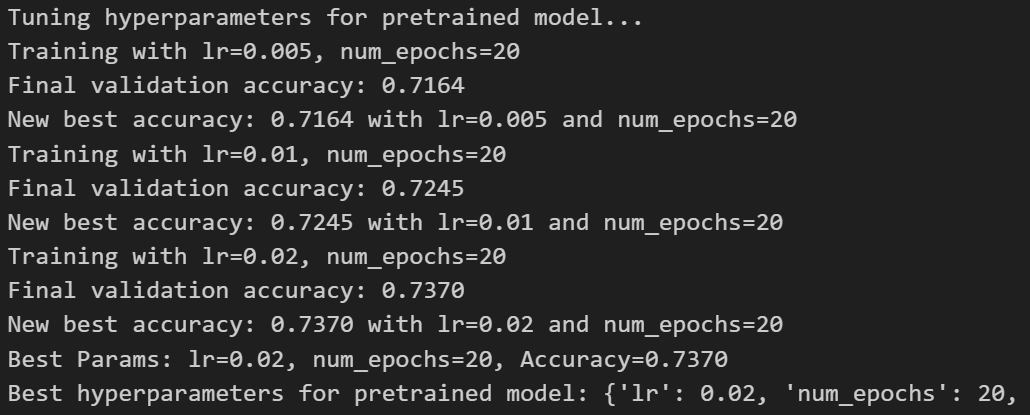
\includegraphics[scale=0.7]{fine.png}
    \caption{最后一次调参结果}
    \label{fig:fine}
\end{figure}

随机初始化模型也可以做调参.本实验中随机初始化模型采用和预训练模型一样的参数,保证比较的公平性.



\section{实验结果}
\subsection{数据分析}
以下图片中,\textcolor{orange}{橙线}都是\textcolor{orange}{预训练模型}的数据曲线,\textcolor{blue}{蓝线}都是\textcolor{blue}{随机初始化模型}的数据曲线.完整的数据文件在文件夹\texttt{run}中.

\begin{figure}[H]
    \centering
    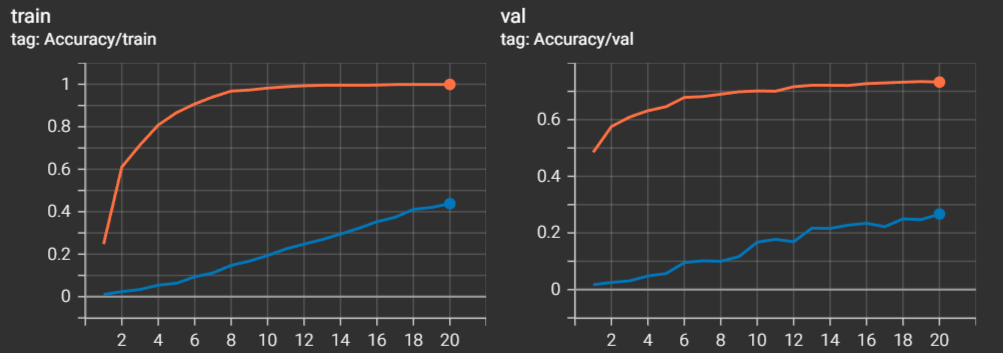
\includegraphics[scale=0.75]{acc.png}
    \caption{准确率对比}
    \label{fig:acc}
\end{figure}

预训练模型的训练准确率迅速上升,并且在初期就已经接近$1$,这表明模型能够很好地学习训练数据.准确率接近1通常表明模型对训练数据的拟合非常好.随机初始化模型的训练准确率相比之下增长较慢,最终也没有接近$1$,这可能意味着模型学习较慢,或者是模型容量不足以完全学习数据.

预训练模型的验证准确率也很快上升并保持在较高水平,这说明预训练模型在未见数据上也具有很好的泛化能力.验证准确率的高稳定性同时也表明模型没有出现显著的过拟合.随机初始化模型的验证准确率虽有所提高,但整体上显著低于预训练模型,这表明其泛化能力较弱.验证准确率的较低水平也表明该模型可能受限于其初始参数设置,未能充分利用训练数据.


\begin{figure}[H]
    \centering
    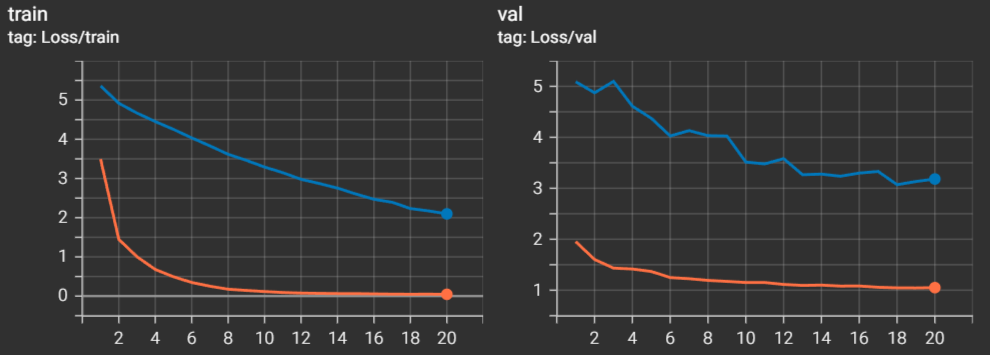
\includegraphics[scale=0.75]{loss.png}
    \caption{损失函数对比}
    \label{fig:loss}
\end{figure}

预训练模型的训练损失迅速下降并趋于平稳,这与高训练准确率一致,表明模型有效地减少了误差.随机初始化模型的训练损失下降较慢,结束时仍高于预训练模型的损失,这进一步证实了其学习效率较低.

预训练模型的验证损失下降并保持较低,与高的验证准确率相符,说明模型在未见数据上的表现良好.验证损失的低水平和稳定性表明没有过拟合.随机初始化模型的验证损失相比之下较高并稍有波动,可能指示模型在未见数据上的性能不够稳定,这可能是由于模型参数初始化不佳或者模型结构不够优化.

\subsection{结论}
预训练模型明显优于随机初始化模型,无论是在训练过程还是在验证过程中.这表明利用预训练的权重可以显著提升模型的学习效率和泛化能力.

随机初始化模型可能需要更多的训练周期、更复杂的网络结构或者更多的调优来提高其性能.

基于以上分析,使用预训练模型在类似的任务中是一个有效的策略,特别是当可用的训练数据量不足以从头训练一个复杂模型时.对于随机初始化的模型,可能需要探索额外的技术,如更深的网络、正则化策略或更精细的超参数调整,以提高其性能.



\chapter{在VOC数据集上训练并测试目标检测模型Faster R-CNN和YOLO V3}
\section{任务描述}
\begin{enumerate}
    \item 学习使用现成的目标检测框架——如mmdetection或detectron2——在VOC数据集上训练并测试目标检测模型Faster R-CNN和YOLO V3;
    \item 挑选4张测试集中的图像,通过可视化对比训练好的Faster R-CNN第一阶段产生的proposal box和最终的预测结果.
    \item 搜集三张不在VOC数据集内包含有VOC中类别物体的图像,分别可视化并比较两个在VOC数据集上训练好的模型在这三张图片上的检测结果(展示bounding box、类别标签和得分)
\end{enumerate}


\section{实验环境}
\subsection{MMDetection 设置:Config is All You Need}
MMDetection 是一个基于 PyTorch 的开源目标检测工具箱,由香港中文大学多媒体实验室(CUHK Multimedia Lab)开发和维护.它是 OpenMMLab 项目的一部分,旨在提供一个灵活、高效、易于使用的目标检测框架,支持各种主流目标检测算法.

MMDetection 对整个目标检测模型的训练流程进行了高程度的封装,用户只需要写出正确的 config 文件而无需过度关注模型训练和测试的工程细节. MMDetection 同时提供了一键部署分布式训练、绘制损失曲线等接口,使得部署十分方便. 本次实验就使用了 mmdet 的相关功能.
\subsection{软硬件环境}

该任务在 \lstinline|Ubuntu 22.04.1 LTS| 上完成,具体如下:

\begin{lstlisting}
    ------------------------------------------------------------
System environment:
    sys.platform: linux
    Python: 3.10.14 (main, May  6 2024, 19:42:50) [GCC 11.2.0]
    CUDA available: True
    MUSA available: False
    numpy_random_seed: 1586568599
    GPU 0,1,2,3: Tesla V100-SXM2-16GB
    CUDA_HOME: /usr/local/cuda-12.0
    NVCC: Cuda compilation tools, release 12.0, V12.0.76
    GCC: gcc (Ubuntu 11.3.0-1ubuntu1~22.04) 11.3.0
    PyTorch: 2.1.2
    PyTorch compiling details: PyTorch built with:
  - GCC 9.3
  - C++ Version: 201703
  - Intel(R) oneAPI Math Kernel Library Version 2023.1-Product Build 20230303 for Intel(R) 64 architecture applications
  - Intel(R) MKL-DNN v3.1.1 (Git Hash 64f6bcbcbab628e96f33a62c3e975f8535a7bde4)
  - OpenMP 201511 (a.k.a. OpenMP 4.5)
  - LAPACK is enabled (usually provided by MKL)
  - NNPACK is enabled
  - CPU capability usage: AVX512
  - CUDA Runtime 11.8
  - NVCC architecture flags: -gencode;arch=compute_50,code=sm_50;-gencode;arch=compute_60,code=sm_60;-gencode;arch=compute_61,code=sm_61;-gencode;arch=compute_70,code=sm_70;-gencode;arch=compute_75,code=sm_75;-gencode;arch=compute_80,code=sm_80;-gencode;arch=compute_86,code=sm_86;-gencode;arch=compute_37,code=sm_37;-gencode;arch=compute_90,code=sm_90;-gencode;arch=compute_37,code=compute_37
  - CuDNN 8.7
  - Magma 2.6.1
  - Build settings: BLAS_INFO=mkl, BUILD_TYPE=Release, CUDA_VERSION=11.8, CUDNN_VERSION=8.7.0, CXX_COMPILER=/opt/rh/devtoolset-9/root/usr/bin/c++, CXX_FLAGS= -D_GLIBCXX_USE_CXX11_ABI=0 -fabi-version=11 -fvisibility-inlines-hidden -DUSE_PTHREADPOOL -DNDEBUG -DUSE_KINETO -DLIBKINETO_NOROCTRACER -DUSE_FBGEMM -DUSE_QNNPACK -DUSE_PYTORCH_QNNPACK -DUSE_XNNPACK -DSYMBOLICATE_MOBILE_DEBUG_HANDLE -O2 -fPIC -Wall -Wextra -Werror=return-type -Werror=non-virtual-dtor -Werror=bool-operation -Wnarrowing -Wno-missing-field-initializers -Wno-type-limits -Wno-array-bounds -Wno-unknown-pragmas -Wno-unused-parameter -Wno-unused-function -Wno-unused-result -Wno-strict-overflow -Wno-strict-aliasing -Wno-stringop-overflow -Wno-psabi -Wno-error=pedantic -Wno-error=old-style-cast -Wno-invalid-partial-specialization -Wno-unused-private-field -Wno-aligned-allocation-unavailable -Wno-missing-braces -fdiagnostics-color=always -faligned-new -Wno-unused-but-set-variable -Wno-maybe-uninitialized -fno-math-errno -fno-trapping-math -Werror=format -Werror=cast-function-type -Wno-stringop-overflow, LAPACK_INFO=mkl, PERF_WITH_AVX=1, PERF_WITH_AVX2=1, PERF_WITH_AVX512=1, TORCH_DISABLE_GPU_ASSERTS=ON, TORCH_VERSION=2.1.2, USE_CUDA=ON, USE_CUDNN=ON, USE_EXCEPTION_PTR=1, USE_GFLAGS=OFF, USE_GLOG=OFF, USE_MKL=ON, USE_MKLDNN=ON, USE_MPI=OFF, USE_NCCL=ON, USE_NNPACK=ON, USE_OPENMP=ON, USE_ROCM=OFF,

    TorchVision: 0.16.2
    OpenCV: 4.9.0
    MMEngine: 0.10.4

Runtime environment:
    cudnn_benchmark: False
    mp_cfg: {'mp_start_method': 'fork', 'opencv_num_threads': 0}
    dist_cfg: {'backend': 'nccl'}
    seed: 1586568599
    Distributed launcher: pytorch
    Distributed training: True
    GPU number: 4
------------------------------------------------------------
\end{lstlisting}

\section{FasterRCNN 实验}

\subsection{实验设置}
在本次实验中,我们在 VOC2007 和 VOC2012 数据集上微调以 ResNet-50 为骨干网络的 FasterRCNN,其预训练权重可以从 \lstinline|torchvision| 中下载:

\begin{lstlisting}[language=Python]
resnet50 = models.resnet50(pretrained=True)
\end{lstlisting}

同时,由于 FasterRCNN 的模型复杂度较高,我们在训练过程中仅对输入图像进行随机翻转这一项噪声加入,最后得到的效果较好.

本次实验在 ROI 头和 RPN 头上都使用了相同的损失函数,其中 bbox 部分使用的是 $L^{1}$-损失函数,分类部分则使用了交叉熵作为损失函数.

训练设置 \lstinline|max_epoch = 10|,但是由于观察到模型在测试集上的表现不再随时间增长,我们在第 7 个轮次结束后便采取了早停措施. \lstinline|batch_size = 8/(per GPU)|,因此总共进行了 10864 次迭代.
\subsection{实验结果}

我们将所有测试中最好的测试结果置于下表,其余的结果可以见于下面的 mAP 曲线和 loss 曲线:

\begin{lstlisting}
    +-------------+------+-------+--------+-------+
    | class       | gts  | dets  | recall | ap    |
    +-------------+------+-------+--------+-------+
    | aeroplane   | 285  | 877   | 0.800  | 0.721 |
    | bicycle     | 337  | 1125  | 0.938  | 0.834 |
    | bird        | 459  | 1159  | 0.874  | 0.784 |
    | boat        | 263  | 1482  | 0.795  | 0.602 |
    | bottle      | 469  | 1340  | 0.642  | 0.527 |
    | bus         | 213  | 938   | 0.930  | 0.833 |
    | car         | 1201 | 3230  | 0.883  | 0.796 |
    | cat         | 358  | 1147  | 0.969  | 0.884 |
    | chair       | 756  | 4585  | 0.860  | 0.632 |
    | cow         | 244  | 921   | 0.934  | 0.830 |
    | diningtable | 206  | 2173  | 0.942  | 0.690 |
    | dog         | 489  | 1527  | 0.969  | 0.862 |
    | horse       | 348  | 1083  | 0.937  | 0.853 |
    | motorbike   | 325  | 1347  | 0.932  | 0.830 |
    | person      | 4528 | 12702 | 0.878  | 0.776 |
    | pottedplant | 480  | 2250  | 0.771  | 0.525 |
    | sheep       | 242  | 733   | 0.876  | 0.750 |
    | sofa        | 239  | 1419  | 0.954  | 0.770 |
    | train       | 282  | 1295  | 0.950  | 0.823 |
    | tvmonitor   | 308  | 1169  | 0.873  | 0.750 |
    +-------------+------+-------+--------+-------+
    | mAP         |      |       |        | 0.754 |
    +-------------+------+-------+--------+-------+
\end{lstlisting}

下图是我们的损失曲线和 mAP 曲线:

\begin{figure}[!htpb]
    \centering
    \begin{minipage}[t]{0.49\textwidth}
    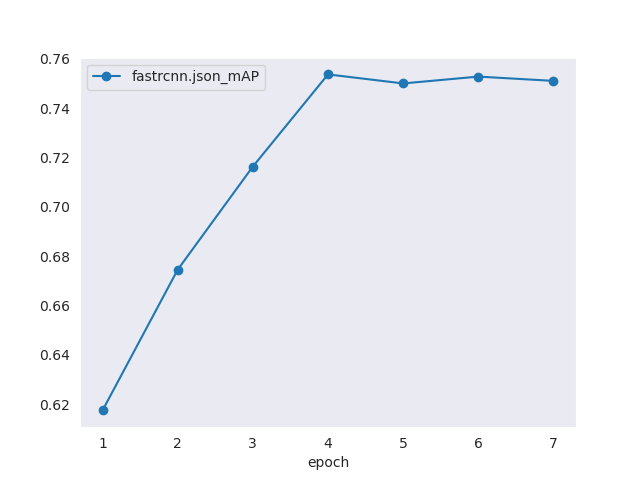
\includegraphics[width=\textwidth]{fastrcnn_mAP.png}
    \caption{FasterRCNN mAP 曲线}
    \label{mAPfrcnn}
    \end{minipage}
    \begin{minipage}[t]{0.49\textwidth}
    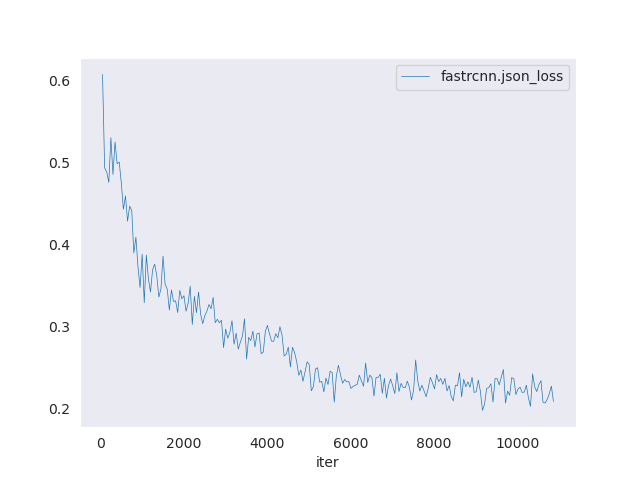
\includegraphics[width=\textwidth]{fastrcnn_loss.png}
    \caption{FasterRCNN 损失函数曲线}
    \label{frcnn_loss}
    \end{minipage}
\end{figure}

\subsection{可视化检测}
我们选取了四张图像,对比了其在 RPN Head 中产生的 proposal box 和最终的预测结果,见下图:
\begin{figure}[!htpb]
    \centering
    \begin{minipage}[t]{0.49\textwidth}
    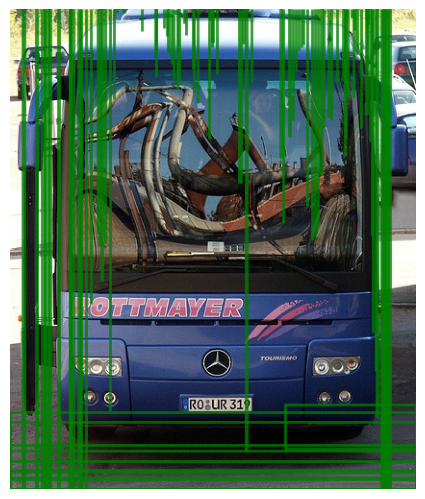
\includegraphics[width=\linewidth]{1ppbox.png}
    \caption{对象1:Proposal Box}
    \label{mAPfrcnn}
    \end{minipage}
    \begin{minipage}[t]{0.49\textwidth}
    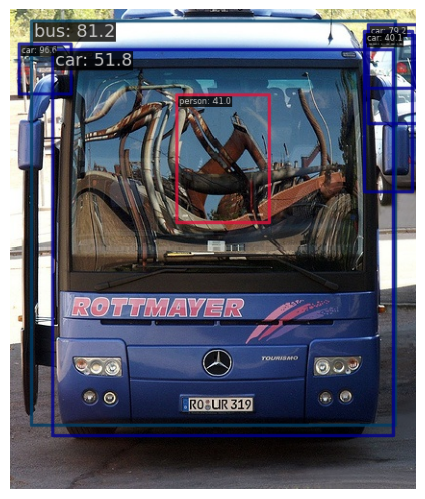
\includegraphics[width=\linewidth]{1result.png}
    \caption{对象1:预测结果}
    \label{frcnn_loss}
    \end{minipage}
\end{figure}
\begin{figure}[!htpb]
    \centering
    \begin{minipage}[t]{0.49\textwidth}
    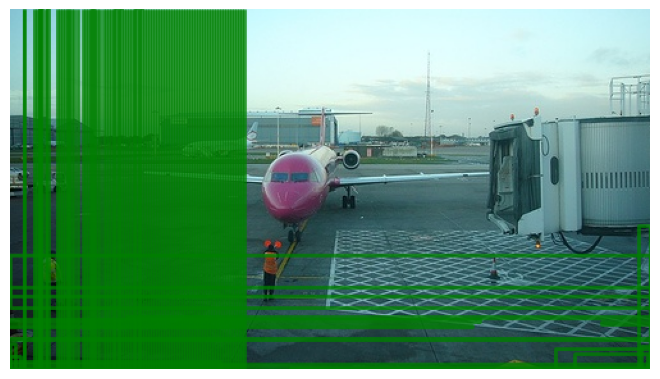
\includegraphics[width=\linewidth]{2ppbox.png}
    \caption{对象2:Proposal Box}
    \label{mAPfrcnn}
    \end{minipage}
    \begin{minipage}[t]{0.49\textwidth}
    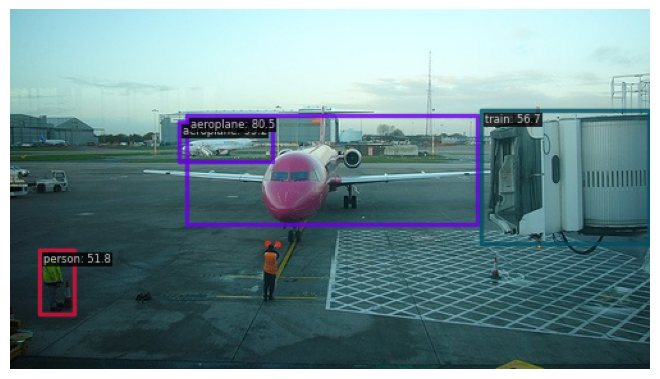
\includegraphics[width=\linewidth]{2result.png}
    \caption{对象2:预测结果}
    \label{frcnn_loss}
    \end{minipage}
\end{figure}

\begin{figure}[!htpb]
    \centering
    \begin{minipage}[t]{0.49\textwidth}
    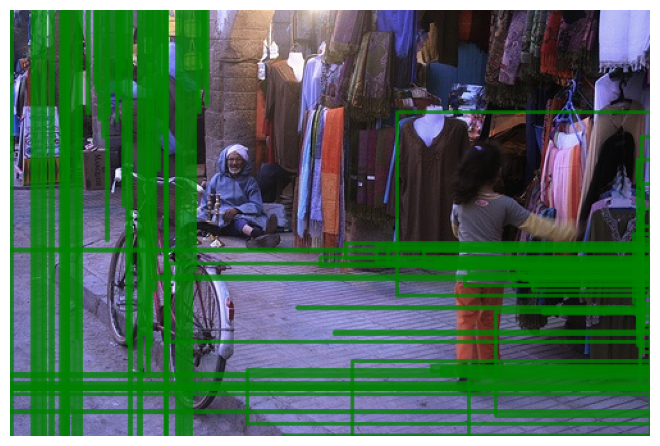
\includegraphics[width=\linewidth]{3ppbox.png}
    \caption{对象3:Proposal Box}
    \label{mAPfrcnn}
    \end{minipage}
    \begin{minipage}[t]{0.49\textwidth}
    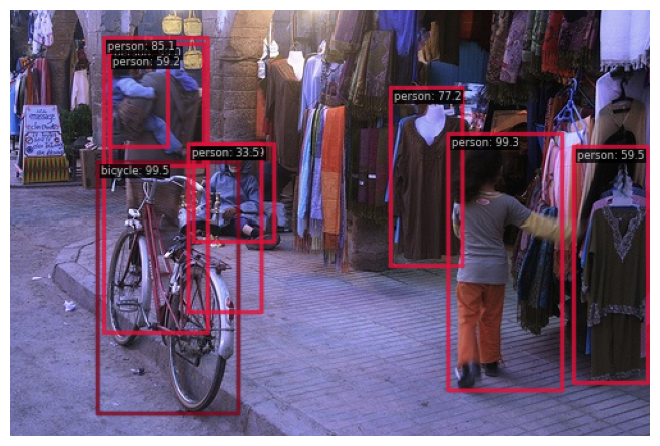
\includegraphics[width=\linewidth]{3result.png}
    \caption{对象3:预测结果}
    \label{frcnn_loss}
    \end{minipage}
\end{figure}
\begin{figure}[!htpb]
    \centering
    \begin{minipage}[t]{0.49\textwidth}
    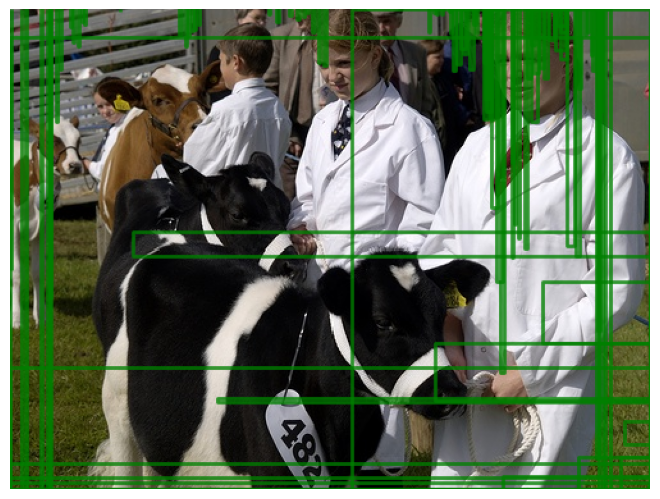
\includegraphics[width=\linewidth]{4ppbox.png}
    \caption{对象4:Proposal Box}
    \label{mAPfrcnn}
    \end{minipage}
    \begin{minipage}[t]{0.49\textwidth}
    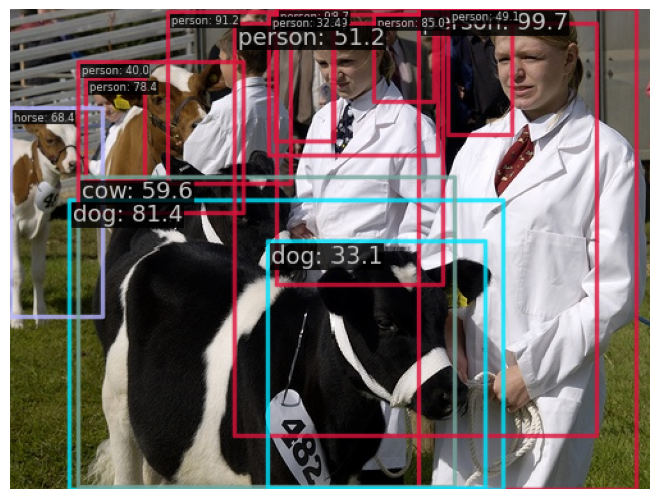
\includegraphics[width=\linewidth]{4result.png}
    \caption{对象4:预测结果}
    \label{frcnn_loss}
    \end{minipage}
\end{figure}

可以看到,通过将RPN Head 的参数\lstinline|num_classes| 设置为 1,Proposal Boxes 较好地完成了区分前后景的任务,最终的 FasterRCNN 预测结果也较为准确.

\subsection{YOLOv3 实验}
\subsection{实验设置}
在本次实验中,我们在 VOC2007 和 VOC2012 数据集上微调以 DarkNet-53 为骨干网络的 YOLOv3,其预训练权重可以从 \lstinline|torchvision| 中下载.

我们的实验重点包括以下两点:

\begin{enumerate}
    \item 数据预处理.
    \item 在实验过程中添加噪声.
\end{enumerate}

在数据预处理部分,我们将每张图像的 RGB 值除以 255,再将图像尺寸填充为能被 32 整除的大小,具体如下:

\begin{lstlisting}[language=Python]
data_preprocessor = dict(
    bgr_to_rgb=True,
    mean=[
        0,
        0,
        0,
    ],
    pad_size_divisor=32,
    std=[
        255.0,
        255.0,
        255.0,
    ],
    type='DetDataPreprocessor')
\end{lstlisting}

实验中添加的噪声则是为了模型的鲁棒性考虑,为了弥补 YOLOv3 的模型差距,在实验中我们采用了更激进的方法向图像增加噪声来进行数据增广,我们使用的方法包括:

\begin{enumerate}
    \item 拓展图像大小
    \item 随机调整图像尺寸
    \item 对图像进行随机裁剪
    \item 对图像进行光度扭曲
    \item 随机翻转图像
\end{enumerate}

同时,在训练中我们还使用了早停机制,当观察到模型在测试集上的 mAP 在几次测试中趋向稳定时,我们提前停止训练,避免模型的过拟合.

和 FasterRCNN 相同,我们使用了 $L^{1}$-损失和交叉熵来作为损失函数.
\subsection{实验结果}

下图是 YOLOv3 训练的 mAP 曲线和 loss 曲线:

\begin{figure}[!htpb]
    \centering
    \begin{minipage}[t]{0.49\textwidth}
    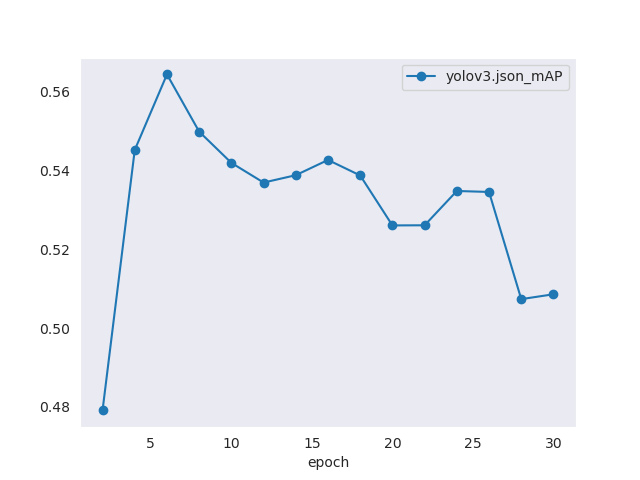
\includegraphics[width=\linewidth]{yolov3_mAP.png}
    \caption{YOLOv3 mAP 曲线}
    \label{mAPfrcnn}
    \end{minipage}
    \begin{minipage}[t]{0.49\textwidth}
    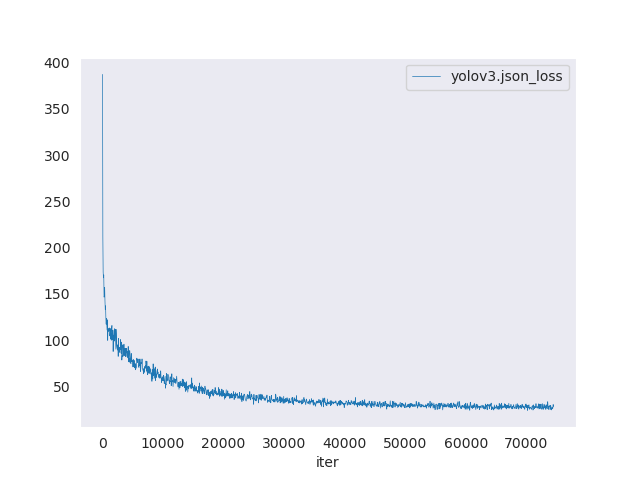
\includegraphics[width=\linewidth]{yolov3_loss.png}
    \caption{YOLOv3 损失函数曲线}
    \label{frcnn_loss}
    \end{minipage}
\end{figure}

YOLOv3 是作者在半夜训练的,所以没有进行早停,实际上通过 mAP 可以发现,训练到第 30 个 epoch 时模型已经严重过拟合.

\section{实验对比}

最后,我们使用不在训练测试集中的三张图片对比 YOLOv3 和 FasterRCNN 的性能.

\begin{figure}[!htpb]
    \centering
    \begin{minipage}[t]{0.49\textwidth}
    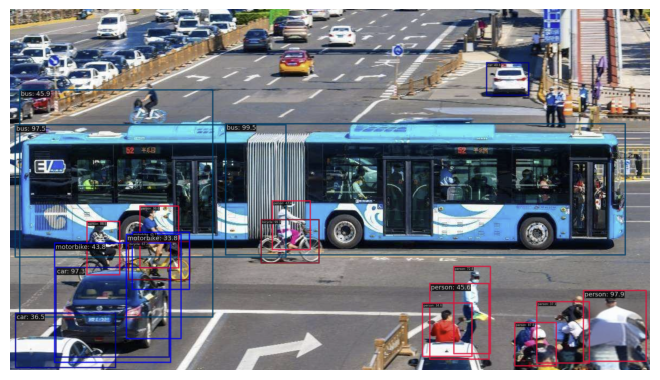
\includegraphics[width=\linewidth]{cnntest1.png}
    \caption{对象1:FasterRCNN 表现}
    \label{mAPfrcnn}
    \end{minipage}
    \begin{minipage}[t]{0.49\textwidth}
    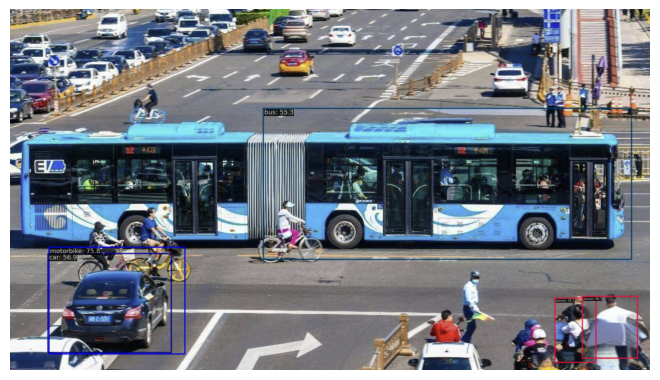
\includegraphics[width=\linewidth]{yolotest1.png}
    \caption{对象1:YOLOv3 表现}
    \label{frcnn_loss}
    \end{minipage}
\end{figure}


\begin{figure}[!htpb]
    \centering
    \begin{minipage}[t]{0.49\textwidth}
    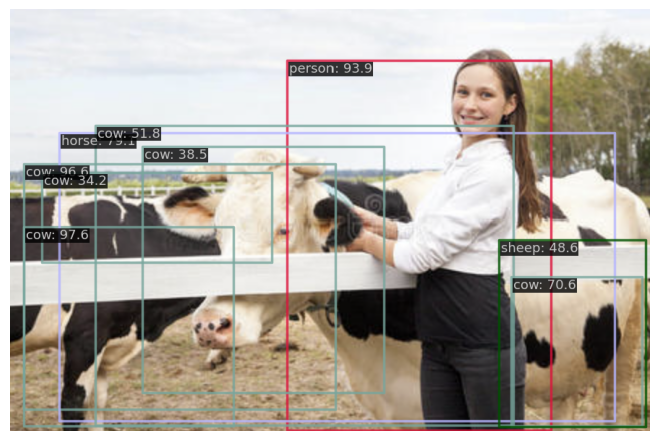
\includegraphics[width=\linewidth]{cnntest2.png}
    \caption{对象2:FasterRCNN 表现}
    \label{mAPfrcnn}
    \end{minipage}
    \begin{minipage}[t]{0.49\textwidth}
        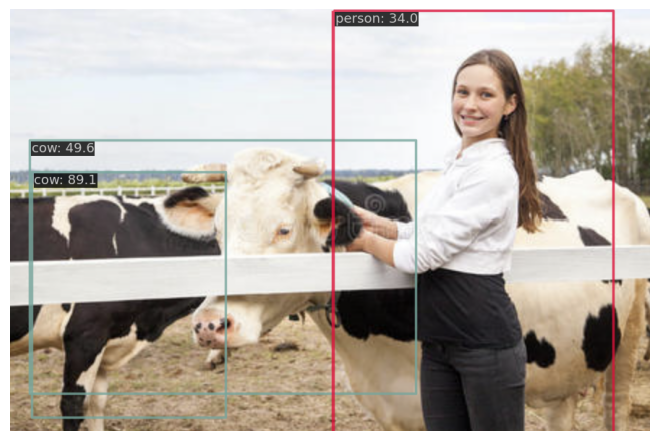
\includegraphics[width=\linewidth]{yolotest2.png}
    \caption{对象2:YOLOv3 表现}
    \label{frcnn_loss}
    \end{minipage}
\end{figure}

\begin{figure}[!htpb]
    \centering
    \begin{minipage}[t]{0.49\textwidth}
    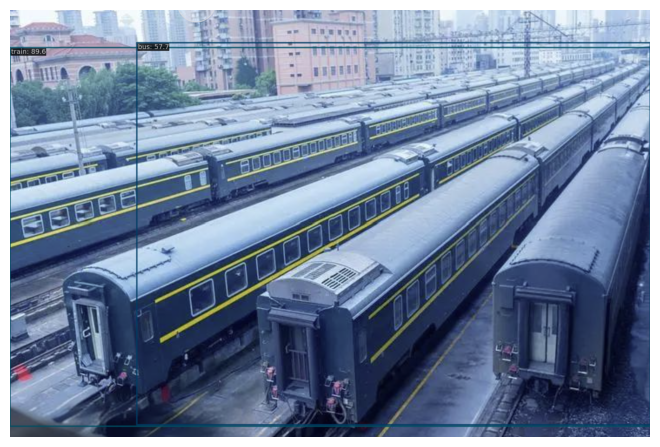
\includegraphics[width=\linewidth]{cnntest3.png}
    \caption{对象3:FasterRCNN 表现}
    \label{mAPfrcnn}
    \end{minipage}
    \begin{minipage}[t]{0.49\textwidth}
    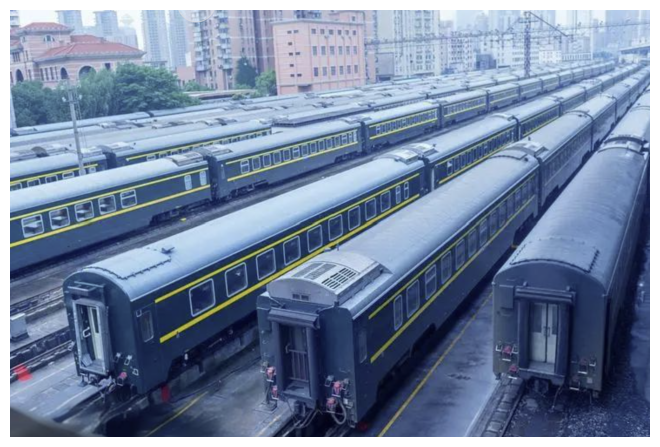
\includegraphics[width=\linewidth]{yolotest3.png}
    \caption{对象3:YOLOv3 表现}
    \label{frcnn_loss}
    \end{minipage}
\end{figure}

可以看到,在识别表现上 YOLOv3 显著落后于 FasterRCNN,在第 3 张实验图像上,YOLOv3 甚至没有识别出火车.

\end{document}
